\documentclass[11pt]{article}
\usepackage{latexsym}
\usepackage{amsmath}
\usepackage{amssymb}
\usepackage{amsthm}
\usepackage{epsfig}
\usepackage{graphicx}
\usepackage{float}
\usepackage{algorithm}
\usepackage{algorithmicx}
\usepackage[noend]{algpseudocode}

\usepackage[shortlabels]{enumitem}

\newcommand{\handout}[5]{
  \noindent
  \begin{center}
  \framebox{
    \vbox{
      \hbox to 5.78in { {\bf ICS 621: Analysis of Algorithms} \hfill #2 }
      \vspace{4mm}
      \hbox to 5.78in { {\Large \hfill #5  \hfill} }
      \vspace{2mm}
      \hbox to 5.78in { {\em #3 \hfill #4} }
    }
  }
  \end{center}
  \vspace*{4mm}
}

\newcommand{\lecture}[4]{\handout{#1}{#2}{#3}{Scribe: #4}{Lecture #1}}

\newtheorem{theorem}{Theorem}
\newtheorem{corollary}[theorem]{Corollary}
\newtheorem{lemma}[theorem]{Lemma}
\newtheorem{observation}[theorem]{Observation}
\newtheorem{proposition}[theorem]{Proposition}
\newtheorem{definition}[theorem]{Definition}
\newtheorem{claim}[theorem]{Claim}
\newtheorem{fact}[theorem]{Fact}
\newtheorem{assumption}[theorem]{Assumption}

% 1-inch margins, from fullpage.sty by H.Partl, Version 2, Dec. 15, 1988.
\topmargin 0pt
\advance \topmargin by -\headheight
\advance \topmargin by -\headsep
\textheight 8.9in
\oddsidemargin 0pt
\evensidemargin \oddsidemargin
\marginparwidth 0.5in
\textwidth 6.5in

\parindent 0in
\parskip 1.5ex
%\renewcommand{\baselinestretch}{1.25}

\newcommand{\VVV}{\mathcal{V}}
\newcommand{\Vor}{\text{Vor}}

\begin{document}

\lecture{12: Interval Trees, Segment Trees}{Fall 2019}{Prof.\ Nodari Sitchinava}{Mojtaba Abolfazli, Muzamil Yahia}

\section{Priority search tree: cont}
\label{sec:range-queries}

This section is the continuation of the last session on Priority Search Trees (PSTs) where we are interested to dive deeper into the analysis of PSTs. Before going into detail, we need to recall PST with $P_{ymax}$ as the point with the largest $y-$coordinate and $x_{med}$ as the median $x$-coordinate among points in database $S$. A PST can be built up as shown in Figure~\ref{fig:PST1} where $S_{left}$ and $S_{right}$ are obtained as follows:
\begin{align*}
    & S_{left}=\{P \in S\setminus \{P_{ymax}\} \mid P.x \leq x_{med} \}\\
    &  S_{right}=\{P \in S\setminus \{P_{ymax}, S_{right}\}\}\\
\end{align*}
\begin{figure}[h!]
\begin{center}
  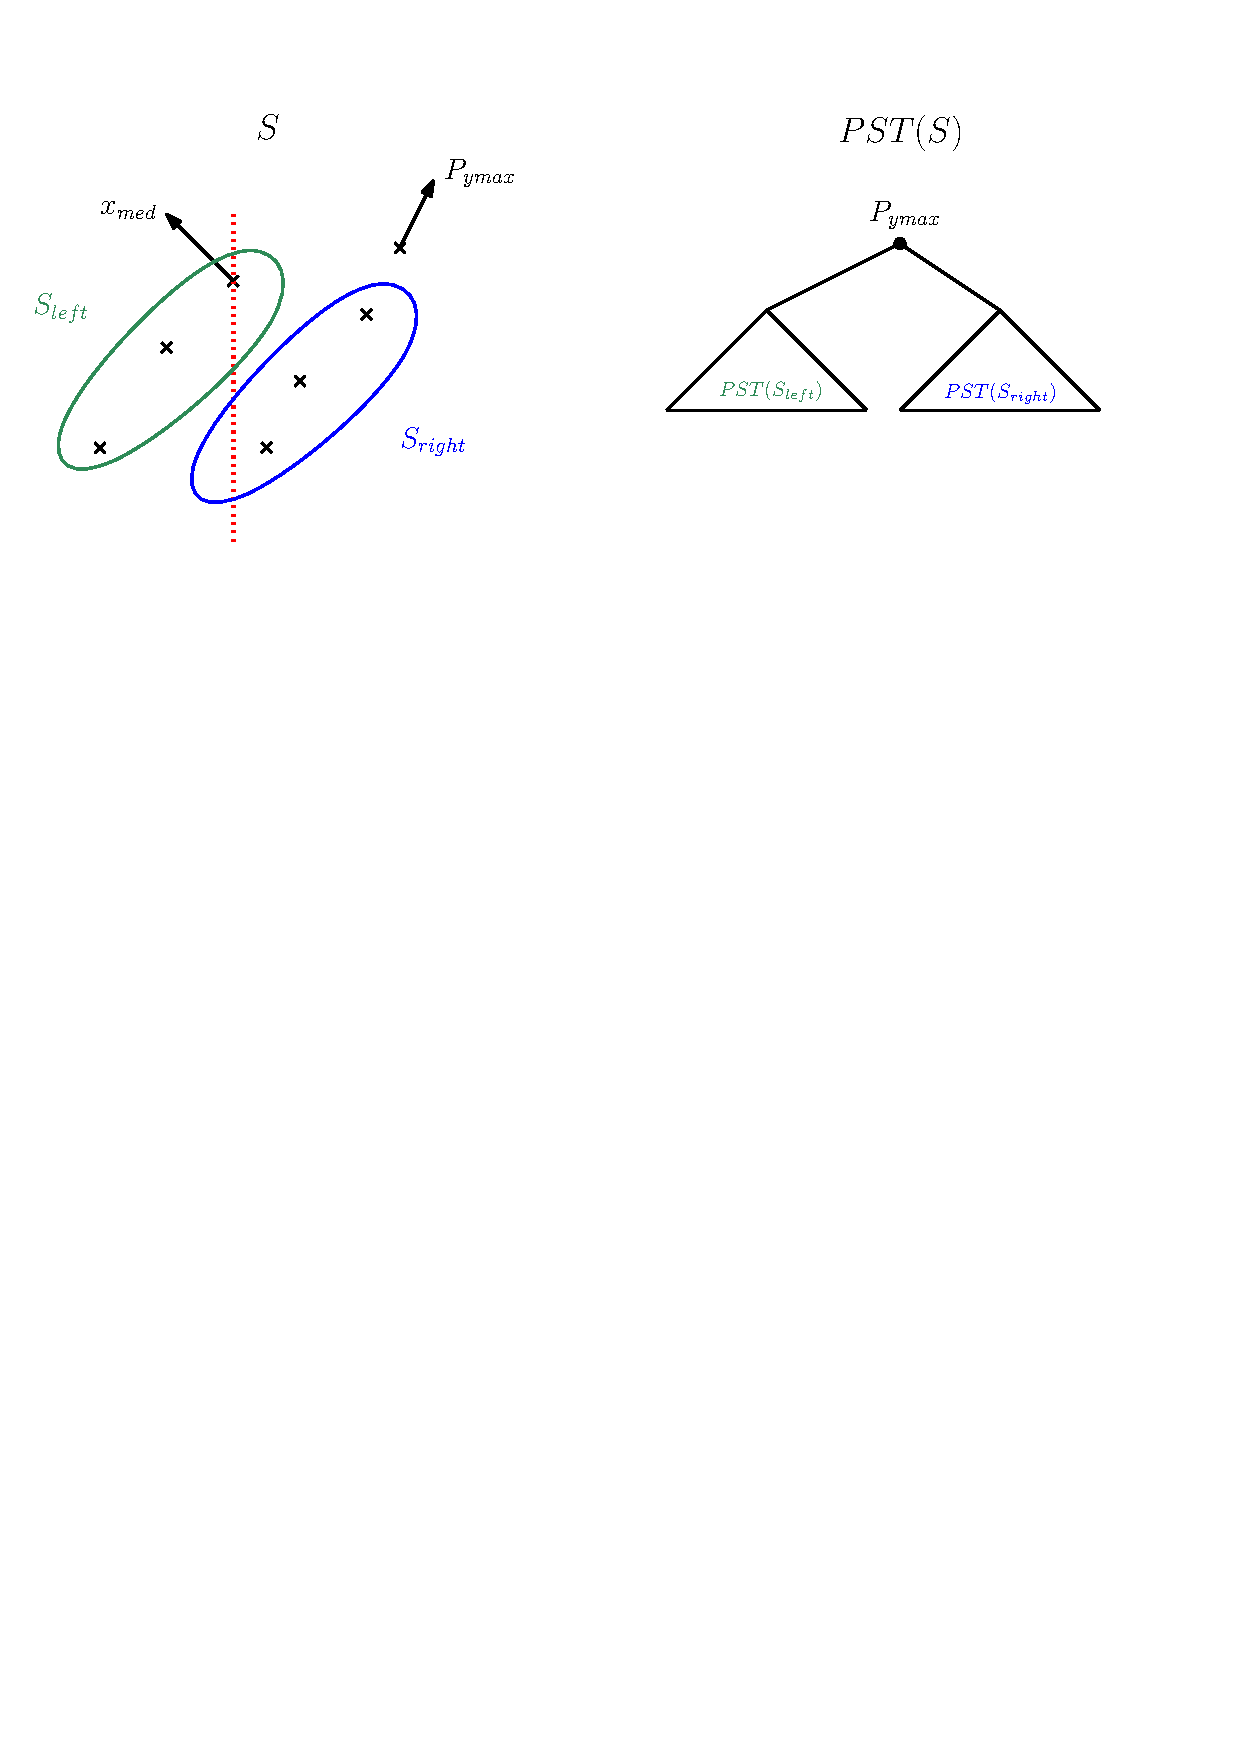
\includegraphics[scale = .5]{ipe/RQ1.pdf}
  \vspace{-0.1in}
  \caption{Building Priority Search Tree.}
  \label{fig:PST1}
\end{center}
\end{figure}

To report all the nodes in a subtree rooted at $v$, we can use the following pseudocode:
\begin{algorithm}[H]
\caption{Report a subtree in PST}\label{Report_subtree1}
\begin{algorithmic}[1]
\Function{Report}{$v$}
\If {$v \neq NULL$}
    \State \Call{Output}{$v$}
    \State \Call{Report}{$v.left$}
    \State \Call{Report}{$v.right$}
\EndIf
\EndFunction
\end{algorithmic}
\end{algorithm}

\subsection{Range Query}
Let's consider a range query in one dimensional space where we're asked to report all points greater than or equal to a real number $q_y$. In this case, we can use the following pseudocode to report all nodes above $q_y$ in a subtree rooted at $v$.
\begin{algorithm}[H]
\caption{Report a subtree above $q_y$ in PST}\label{Report_subtree2}
\begin{algorithmic}[1]
\Function{Report}{$v, q_y$}
\If {$v \neq NULL$}
    \If {$v.y \geq q_y$}
        \State \Call{Output}{$v$}
        \State \Call{Report}{$v.left, q_y$}
        \State \Call{Report}{$v.right, q_y$}
    \EndIf
\EndIf
\EndFunction
\end{algorithmic}
\end{algorithm}
The above pseudocode reports all the points above $q_y$ because any path from root $v$ to any node is in a non-decreasing order of $y-$coordinate (otherwise the property of PST doesn't hold). Likewise, the subtree of nodes needs to be reported is either connected and contains the root or it is empty.

The performance of PSTs is summarized in the following theorem.
\begin{theorem}\label{theorem1:RQ}
The total running time to report all points in a query range $[q_y, +\infty]$ in a PST rooted at $v$ is:
\begin{equation*}
    T(v) = c\cdot k_v + c - 1
\end{equation*}
where $k_v$ is the number of reported points and $c \geq 1$.
\end{theorem}

\begin{proof}
We prove the theorem by using the induction.\\
\textit{Induction hypothesis:} For all descendant nodes $u$ of $v$:
\begin{equation*}
    T(u) = c\cdot k_u + c-1
\end{equation*}
where $k_u$ is the total number of nodes above $q_y$ in a PST rooted at $u$.\\

For the base case where there is no point in the query above $q_y$, the theorem is true. Now we show that it's also true for the PST rooted at $v$.
\begin{align*}
    T(v) &= 1 + T(v.left)+ T(v.right)\\
    &= 1 + c\cdot k_{v.left} + c-1 + c\cdot k_{v.right} + c-1 \\
    &= c-1 + c(1+k_{v.left}+k_{v.right})\\
    &= c-1 + c\cdot k_v
\end{align*}
\end{proof}

\subsection{3-sided Range Query}

Now, let's look at 2D range query where we aim to find nodes within a 3-sided range (i.e. $[x_L, x_R] \times [y, +\infty]$) as shown in Figure~\ref{fig:PST2}.
\begin{figure}[h!]
\begin{center}
  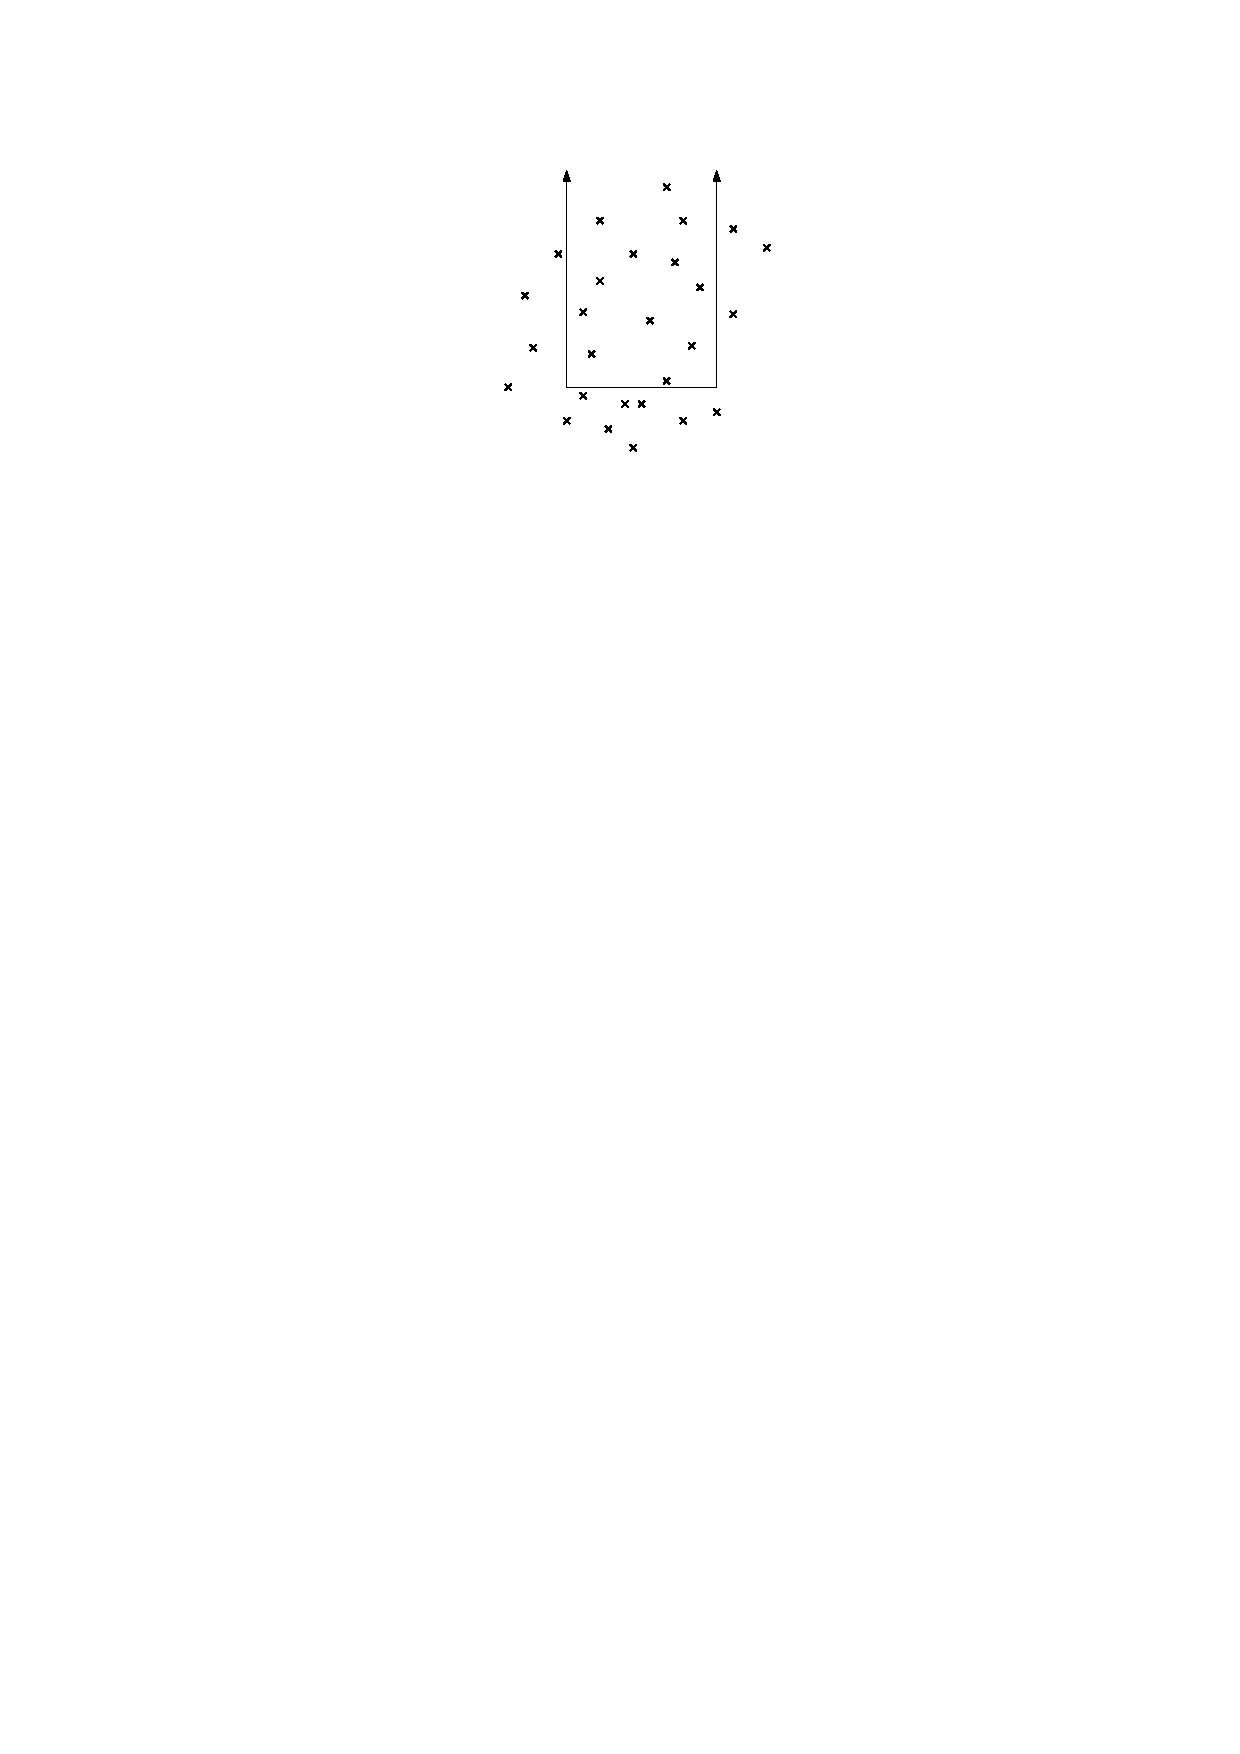
\includegraphics[scale = 1]{ipe/RQ2.pdf}
  \vspace{-0.1in}
  \caption{3-sided Range Query.}
  \label{fig:PST2}
\end{center}
\end{figure}


We follow the subsequent steps to report all nodes corresponding to the specified range:
\begin{itemize}
    \item Find splitting vertex $v_{split}$.
    \item Follow left path down to $x_L$ (left boundary) and report all points in the subtrees hanging from the right.
    \item Follow right path down to $x_R$ (right boundary) and report all points in the subtrees hanging from the left.
\end{itemize}
The following pseudocode describes the query algorithm:

\begin{algorithm}[h!]
\caption{3-sided Range Query}\label{3-sided}
\begin{algorithmic}[1]
\Function{3-sided Query}{$v, [x_L, x_R], y$}
\While{$(v \neq NULL) \textbf{and} (v.x_{med} \leq x_L \ \textbf{or} \ x_R < v.x_{med})$}
    \If {$v \in [x_L, x_R] \times [y, +\infty]$}
        \State \Call{Output}{$v$}
    \EndIf
    \If {$v.x_{med} \leq x_L$}
        \State {$v = v.right $}
    \Else
        \State {$v = v.left $}
    \EndIf
    \State {$v_{split} = v$}
    \State {$v = v.left$}
    \If {$v_{split} \in [x_L, x_R] \times [y, +\infty]$}
        \State \Call{Output}{$v_{split}$}
    \EndIf
\EndWhile
\While{$v \neq NULL$}
    \If {$v \in [x_L, x_R] \times [y, +\infty]$}
        \State \Call{Output}{$v$}
    \EndIf
    \If {$x_L \leq v.x_{med}$}
        \State \Call{Report}{$v.right, y$}
        \State {$v = v.left$}
    \Else
        \State {$v = v.right $}
    \EndIf
    \State {$v = v_{split}.right$}
\EndWhile

\While{$v \neq NULL$}
    \If {$v \in [x_L, x_R] \times [y, +\infty]$}
        \State \Call{Output}{$v$}
    \EndIf
    \If {$v.x_{med} \leq x_R$}
        \State \Call{Report}{$v.left, y$}
        \State {$v = v.right$}
    \Else
        \State {$v = v.left $}
    \EndIf
\EndWhile
\EndFunction
\end{algorithmic}
\end{algorithm}

We start to find the splitting point with $x_L$ and $x_R$ as shown in Figure~\ref{fig:PST3}. All shaded subtrees are those whose $x-$coordinate lies in the specified range. Therefore, we can search those subtrees based on just $y-$coordinate as given in Algorithm~\ref{Report_subtree2}. 

\begin{figure}[h!]
\begin{center}
  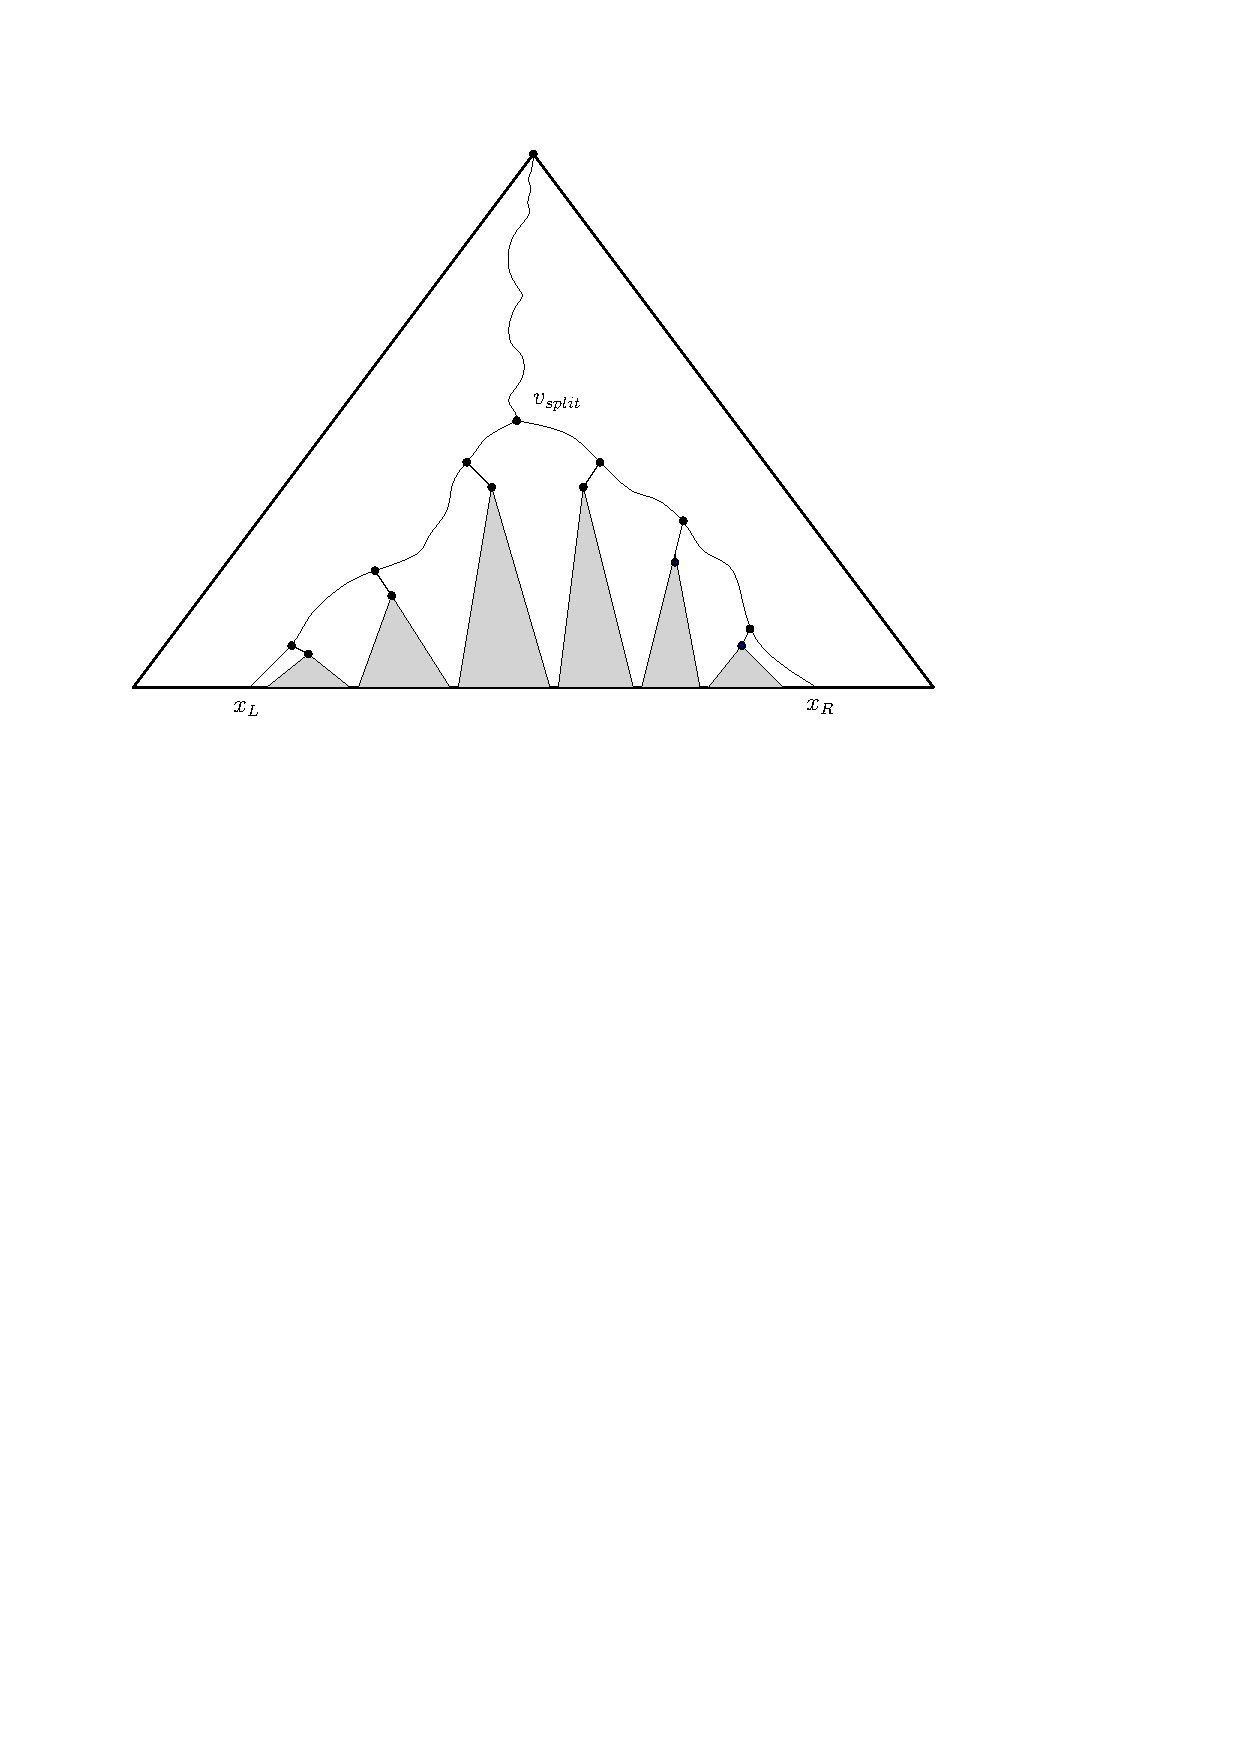
\includegraphics[scale = .5]{ipe/RQ3.pdf}
  \vspace{-0.1in}
  \caption{Querying a PST.}
  \label{fig:PST3}
\end{center}
\end{figure}

As discussed in the previous session, the running time for 2D query is of the order $T(v) = O(\log n+k)$ where $k$ denote the number of reported points. The PST for $n$ points uses $O(n \log n)$ memory space to store the data and takes $O(n \log n)$ to build.

\section{Interval trees for orthogonal stabbing queries}
\label{sec:interval-trees}

In certain geometric applications like planar graphs, we might be interested in reporting the set of line segments $L$ associated with a window query  $w = [x_0, x_1] \times [y_0, y_1]$. 
%
This set $L$ contains all line segments with at least one end point inside $w$, or those segments that pass through the window $w$. 

We can report all line segments with at least one endpoint inside $w$ using algorithms and techniques from Section \ref{sec:range-queries}. 
%
We can use 2 instances of 3-sided query i.e. $ q_0 = [x_0, x_1] \times [y_0, +\infty ]  $ and $q_1 = [x_0, x_1] \times [-\infty,y_1]$, and then report the intersections of the two queries in time $O(\log n + k_0) + O(\log n + k_1) $. 
%
However, in the worst case scenario, the two queries may report all $n = k_0 + k_1$ endpoints while the intersection may contain only one element.
%
By constructing 2D range trees with storage $O(n\log n)$, and time $O(\log^2 n + k)$ we can report all line segments with ends points in $w$. Applying fractional cascading can reduce the query time further to $O(\log n +k)$ which is faster than $(\log n + n)$.

What is left is how to handle efficiently those line segments that pass through our window query $w$? In other words, we are looking for line segments that stab two boundaries of our window query $w$. If we know how to report all line segments that stab one boundary,  say $[x_0, x_1]$, of $w$, we can easily check if they stab any of the remaining boundaries. In this section, we present a data structure that can handle stabbing queries for orthogonal line segments in $O(\log n + k)$ time, and in the next section, we show how report stabbing queries for slanted line segments in $O(\log n + k)$. 

ADD PICTURE HERE OF WINDOW QUERY


\section{Segment trees for stabbing queries}
\label{sec:segmenet-trees}

Consider the set of line segments $L = \{ \ell_1, \ell_2, \ell_3, \ell_4, \ell_5\}$ in the following diagrams: 

\begin{figure}[h!]
\centering
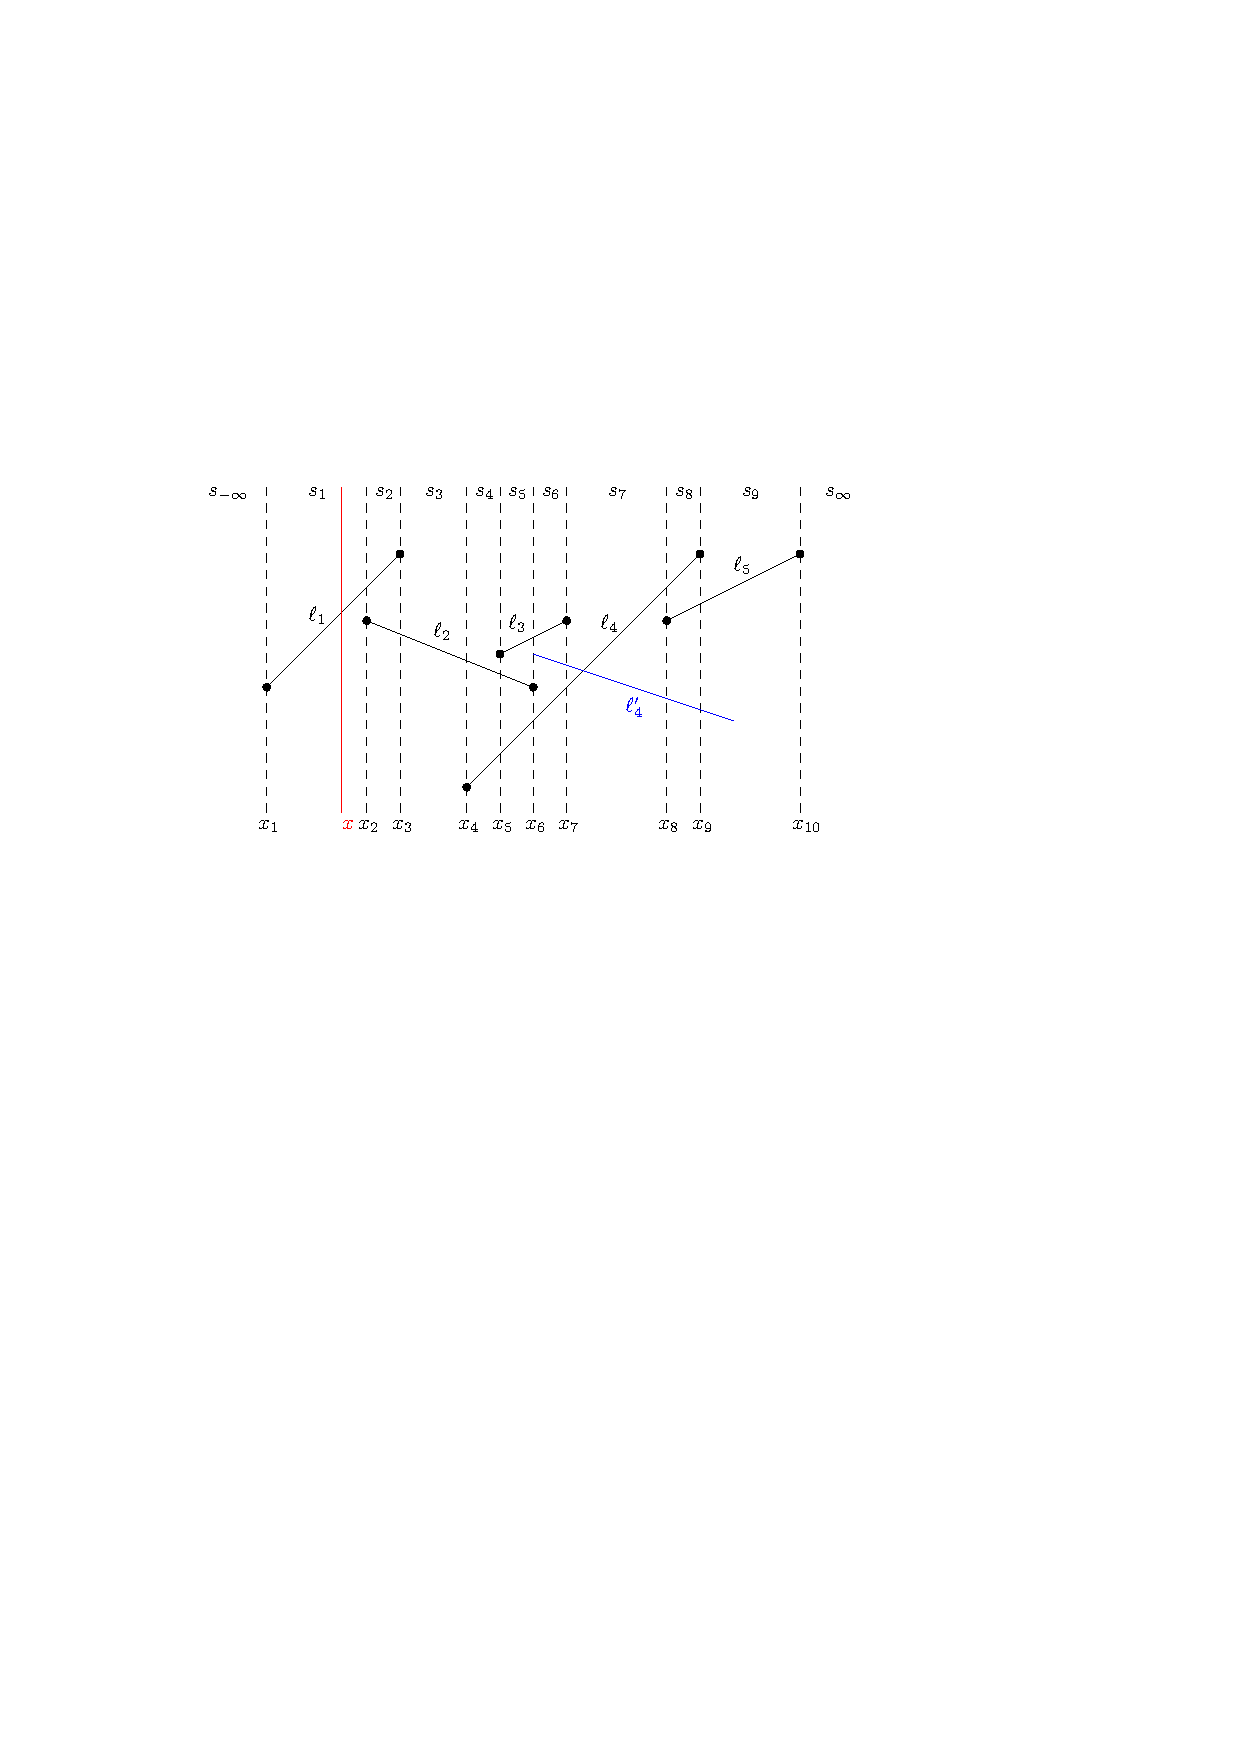
\includegraphics[scale = .8]{ipe/slanted-lines.pdf}
\caption{Set of line segments $L = \{ \ell_1, \ell_2, \ell_3, \ell_4, \ell_5\}$ with slabs $S = \{s_{-\infty},s_1, \dots, s_9, s_{\infty} \}$.}
\end{figure}
Observe that we can't always define a total ordering over slanted line segments that preserves the transitivity property. 
%
For example, if we consider $\ell_5 \leq \ell_4 \leq \ell_2$ then by transitivity we would have $\ell_5 \leq \ell_2$. 
%
On the other hand, if we consider $\ell_2 \leq \textcolor{red}{\ell'_4} \leq \ell_5$ then we would have $\ell _2 \leq \ell_5$. 
%
However, if we divide the plane into slabs shown by the dashed lines, we can define a total ordering within each slab that is transitive. 

We can build a BST for slabs based on $x$-values of end points with leaves $S = \{s_{-\infty},s_1, \dots, s_9, s_{\infty} \}$, and internal node $v$ being the union of all slabs within the subtree rooted at $v$. 
%
The root is then all $x$-axis given by the only slab $[-\infty, \infty]$.
%
Next we augment the BST node $v$ with list of line segments $\ell$ that crosses any slab with its subtree but do not cross the parent slab. 
%
\paragraph{Invariant} Each line segment $\ell$ is stored in a node of $v$ such that 
\[ [v.x_{left}, v.x_{right}] \subseteq [ \ell.x_{left}, \ell.x_{right}]   \; \wedge \; [parent(v).x_{left}, parent(v).x_{right}] \not \subseteq [\ell.x_{left}, \ell.x_{right}].   \]

\begin{claim}
Each segment will be stored in at most 2 nodes at each level of segment tree.
\end{claim} 

The proof of the claim above can be found in chapter 10 in \cite{Berg:2008}. Based on the result above, the segment tree would take $O(n \log n)$ space and answer stabbing queries in $O(\log n + k)$.

\bibliography{biblio}
\bibliographystyle{alpha}

\end{document}
